% Options for packages loaded elsewhere
\PassOptionsToPackage{unicode}{hyperref}
\PassOptionsToPackage{hyphens}{url}
\PassOptionsToPackage{dvipsnames,svgnames,x11names}{xcolor}
%
\documentclass[
  letterpaper,
  DIV=11,
  numbers=noendperiod]{scrreprt}

\usepackage{amsmath,amssymb}
\usepackage{iftex}
\ifPDFTeX
  \usepackage[T1]{fontenc}
  \usepackage[utf8]{inputenc}
  \usepackage{textcomp} % provide euro and other symbols
\else % if luatex or xetex
  \usepackage{unicode-math}
  \defaultfontfeatures{Scale=MatchLowercase}
  \defaultfontfeatures[\rmfamily]{Ligatures=TeX,Scale=1}
\fi
\usepackage{lmodern}
\ifPDFTeX\else  
    % xetex/luatex font selection
\fi
% Use upquote if available, for straight quotes in verbatim environments
\IfFileExists{upquote.sty}{\usepackage{upquote}}{}
\IfFileExists{microtype.sty}{% use microtype if available
  \usepackage[]{microtype}
  \UseMicrotypeSet[protrusion]{basicmath} % disable protrusion for tt fonts
}{}
\makeatletter
\@ifundefined{KOMAClassName}{% if non-KOMA class
  \IfFileExists{parskip.sty}{%
    \usepackage{parskip}
  }{% else
    \setlength{\parindent}{0pt}
    \setlength{\parskip}{6pt plus 2pt minus 1pt}}
}{% if KOMA class
  \KOMAoptions{parskip=half}}
\makeatother
\usepackage{xcolor}
\setlength{\emergencystretch}{3em} % prevent overfull lines
\setcounter{secnumdepth}{5}
% Make \paragraph and \subparagraph free-standing
\ifx\paragraph\undefined\else
  \let\oldparagraph\paragraph
  \renewcommand{\paragraph}[1]{\oldparagraph{#1}\mbox{}}
\fi
\ifx\subparagraph\undefined\else
  \let\oldsubparagraph\subparagraph
  \renewcommand{\subparagraph}[1]{\oldsubparagraph{#1}\mbox{}}
\fi


\providecommand{\tightlist}{%
  \setlength{\itemsep}{0pt}\setlength{\parskip}{0pt}}\usepackage{longtable,booktabs,array}
\usepackage{calc} % for calculating minipage widths
% Correct order of tables after \paragraph or \subparagraph
\usepackage{etoolbox}
\makeatletter
\patchcmd\longtable{\par}{\if@noskipsec\mbox{}\fi\par}{}{}
\makeatother
% Allow footnotes in longtable head/foot
\IfFileExists{footnotehyper.sty}{\usepackage{footnotehyper}}{\usepackage{footnote}}
\makesavenoteenv{longtable}
\usepackage{graphicx}
\makeatletter
\def\maxwidth{\ifdim\Gin@nat@width>\linewidth\linewidth\else\Gin@nat@width\fi}
\def\maxheight{\ifdim\Gin@nat@height>\textheight\textheight\else\Gin@nat@height\fi}
\makeatother
% Scale images if necessary, so that they will not overflow the page
% margins by default, and it is still possible to overwrite the defaults
% using explicit options in \includegraphics[width, height, ...]{}
\setkeys{Gin}{width=\maxwidth,height=\maxheight,keepaspectratio}
% Set default figure placement to htbp
\makeatletter
\def\fps@figure{htbp}
\makeatother
\newlength{\cslhangindent}
\setlength{\cslhangindent}{1.5em}
\newlength{\csllabelwidth}
\setlength{\csllabelwidth}{3em}
\newlength{\cslentryspacingunit} % times entry-spacing
\setlength{\cslentryspacingunit}{\parskip}
\newenvironment{CSLReferences}[2] % #1 hanging-ident, #2 entry spacing
 {% don't indent paragraphs
  \setlength{\parindent}{0pt}
  % turn on hanging indent if param 1 is 1
  \ifodd #1
  \let\oldpar\par
  \def\par{\hangindent=\cslhangindent\oldpar}
  \fi
  % set entry spacing
  \setlength{\parskip}{#2\cslentryspacingunit}
 }%
 {}
\usepackage{calc}
\newcommand{\CSLBlock}[1]{#1\hfill\break}
\newcommand{\CSLLeftMargin}[1]{\parbox[t]{\csllabelwidth}{#1}}
\newcommand{\CSLRightInline}[1]{\parbox[t]{\linewidth - \csllabelwidth}{#1}\break}
\newcommand{\CSLIndent}[1]{\hspace{\cslhangindent}#1}

\KOMAoption{captions}{tableheading}
\makeatletter
\makeatother
\makeatletter
\@ifpackageloaded{bookmark}{}{\usepackage{bookmark}}
\makeatother
\makeatletter
\@ifpackageloaded{caption}{}{\usepackage{caption}}
\AtBeginDocument{%
\ifdefined\contentsname
  \renewcommand*\contentsname{Table of contents}
\else
  \newcommand\contentsname{Table of contents}
\fi
\ifdefined\listfigurename
  \renewcommand*\listfigurename{List of Figures}
\else
  \newcommand\listfigurename{List of Figures}
\fi
\ifdefined\listtablename
  \renewcommand*\listtablename{List of Tables}
\else
  \newcommand\listtablename{List of Tables}
\fi
\ifdefined\figurename
  \renewcommand*\figurename{Figure}
\else
  \newcommand\figurename{Figure}
\fi
\ifdefined\tablename
  \renewcommand*\tablename{Table}
\else
  \newcommand\tablename{Table}
\fi
}
\@ifpackageloaded{float}{}{\usepackage{float}}
\floatstyle{ruled}
\@ifundefined{c@chapter}{\newfloat{codelisting}{h}{lop}}{\newfloat{codelisting}{h}{lop}[chapter]}
\floatname{codelisting}{Listing}
\newcommand*\listoflistings{\listof{codelisting}{List of Listings}}
\makeatother
\makeatletter
\@ifpackageloaded{caption}{}{\usepackage{caption}}
\@ifpackageloaded{subcaption}{}{\usepackage{subcaption}}
\makeatother
\makeatletter
\@ifpackageloaded{tcolorbox}{}{\usepackage[skins,breakable]{tcolorbox}}
\makeatother
\makeatletter
\@ifundefined{shadecolor}{\definecolor{shadecolor}{rgb}{.97, .97, .97}}
\makeatother
\makeatletter
\makeatother
\makeatletter
\makeatother
\ifLuaTeX
  \usepackage{selnolig}  % disable illegal ligatures
\fi
\IfFileExists{bookmark.sty}{\usepackage{bookmark}}{\usepackage{hyperref}}
\IfFileExists{xurl.sty}{\usepackage{xurl}}{} % add URL line breaks if available
\urlstyle{same} % disable monospaced font for URLs
\hypersetup{
  pdftitle={The Little Book of Smiley Plots},
  pdfauthor={The SPAAM Community},
  colorlinks=true,
  linkcolor={blue},
  filecolor={Maroon},
  citecolor={Blue},
  urlcolor={Blue},
  pdfcreator={LaTeX via pandoc}}

\title{The Little Book of Smiley Plots}
\usepackage{etoolbox}
\makeatletter
\providecommand{\subtitle}[1]{% add subtitle to \maketitle
  \apptocmd{\@title}{\par {\large #1 \par}}{}{}
}
\makeatother
\subtitle{A collection of ancient DNA patterns and their causes}
\author{The SPAAM Community}
\date{2025-01-05}

\begin{document}
\maketitle
\ifdefined\Shaded\renewenvironment{Shaded}{\begin{tcolorbox}[borderline west={3pt}{0pt}{shadecolor}, frame hidden, sharp corners, enhanced, breakable, interior hidden, boxrule=0pt]}{\end{tcolorbox}}\fi

\renewcommand*\contentsname{Table of contents}
{
\hypersetup{linkcolor=}
\setcounter{tocdepth}{2}
\tableofcontents
}
\bookmarksetup{startatroot}

\hypertarget{preface}{%
\chapter*{Preface}\label{preface}}
\addcontentsline{toc}{chapter}{Preface}

\markboth{Preface}{Preface}

A key part of any ancient DNA project is to show that the DNA is exactly
that - that the DNA is ancient, rather than from modern contamination.

A key authentication method is to show the presence of elevated C to T
deamination patterns (and the complementary G to A) at the end of DNA
molecules - known as damage patterns - originally reported by (Briggs et
al. 2007).

These patterns can be plotted in what have been colloquially known as
'Smiley Plots. However, there can be a wide range of smiley plots, some
which show valid ancient DNA, and others that do not - either due to not
actually having true ancient DNA but also from laboratory and/or
bioinformatic artifacts.

This book aims to act as a reference guide to interpreting ancient DNA
damage plots, providing a wide range of example `smiley plots', with
descriptions of what the describe and what can cause them. As an added
bit of fun, each type of `smiley plot' comes with a artistic
interpretation of the line shape contributed by members of the ancient
DNA community.

\bookmarksetup{startatroot}

\hypertarget{introduction}{%
\chapter*{Introduction}\label{introduction}}
\addcontentsline{toc}{chapter}{Introduction}

\markboth{Introduction}{Introduction}

\hypertarget{what-are-damage-patterns}{%
\section*{What are damage patterns?}\label{what-are-damage-patterns}}
\addcontentsline{toc}{section}{What are damage patterns?}

\markright{What are damage patterns?}

Damage patterns on ancient DNA molecules occur due to increased
miscoding lesions at the end of molecules. When DNA molecules start to
decompose (i.e., repair mechanisms are lost once an organism dies), the
very long DNA molecules start to fragment due to `nicks' occurring on
the sugar-phosphate of one of the strands, weakening the structure and
causing the molecule to cleave into two. However, this cleavage is not
necessarily `clean', i.e., occurs on both strands at the same position.
Rather, when the two uneven `nicks' cause the DNA molecule to cleave
into two, this results in a `jagged' break - with the molecules having
`overhangs' of one strand being longer than the other of each of the new
two now-`independent' molecules.

The resulting single-stranded overhangs leave the nitrogenous-bases
`exposed' on the overhang to the surrounding environment. It was found

It is important to note that the library construction method will
influence damage, e.g., is the library constructed from double-stranded
DNA or single-stranded DNA, is the polymerase in the initial library
amplification proof-reading or not, and so on.

Figure~\ref{fig-briggs-2007}

\begin{figure}

{\centering 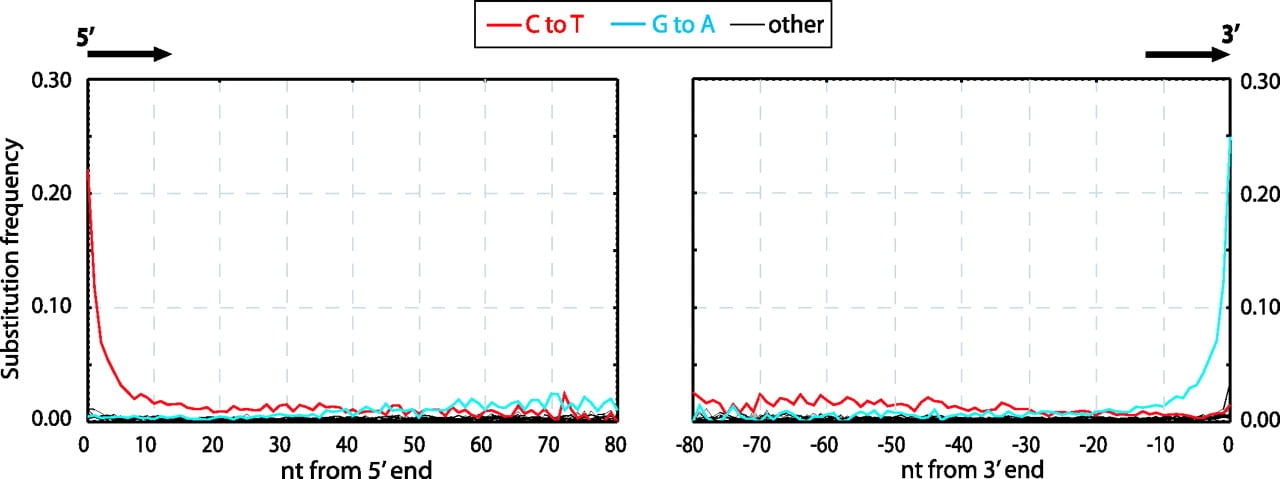
\includegraphics{assets/images/briggs_2007_original_Damage_pattern.jpeg}

}

\caption{\label{fig-briggs-2007}First reported misincorporation lesion
`smiley plot' from Neanderthal DNA (Briggs et al. 2007). Reproduced here
under free access.}

\end{figure}

\hypertarget{how-to-generate-damage-patterns}{%
\section*{How to generate damage
patterns}\label{how-to-generate-damage-patterns}}
\addcontentsline{toc}{section}{How to generate damage patterns}

\markright{How to generate damage patterns}

There is a range of software that can generate damage pattern plots from
ancient DNA NGS libraries. The vast majority of tools require to be of
sequencing reads aligned to a reference genome. Here we make suggestions
of some tools that you can use to generate such plots.

\hypertarget{genomics}{%
\subsection*{Genomics}\label{genomics}}
\addcontentsline{toc}{subsection}{Genomics}

These tools general take BAM files as input (i.e., after mapping of
FASTQ files to a reference genome using a short-read aligner )

\begin{itemize}
\tightlist
\item
  mapDamage

  \begin{itemize}
  \tightlist
  \item
    Source:
    \href{https://github.com/ginolhac/mapDamage}{https://github.com/ginolhac/mapDamagee}
  \item
    Documentation: \url{https://ginolhac.github.io/mapDamage}
  \item
    Citation: (Jónsson et al. 2013)
  \end{itemize}
\item
  DamageProfiler

  \begin{itemize}
  \tightlist
  \item
    Source:
    \url{https://github.com/Integrative-Transcriptomics/DamageProfiler}
  \item
    Documentation:
    \url{https://damageprofiler.readthedocs.io/en/latest/}
  \item
    Citation: (Neukamm, Peltzer, and Nieselt 2021)
  \end{itemize}
\end{itemize}

\hypertarget{metagenomics}{%
\subsection*{Metagenomics}\label{metagenomics}}
\addcontentsline{toc}{subsection}{Metagenomics}

\begin{itemize}
\tightlist
\item
  MaltExtract

  \begin{itemize}
  \tightlist
  \item
    Source: \url{https://github.com/rhuebler/MaltExtract}
  \item
    Documentation: \url{https://github.com/rhuebler/MaltExtract}
  \item
    Citation: (Hübler et al. 2019)
  \end{itemize}
\end{itemize}

\part{Valid Smiley Plots}

\hypertarget{smiley-pplot-of-double-stranded-dna-libraries}{%
\chapter{Smiley pplot of double stranded DNA
libraries}\label{smiley-pplot-of-double-stranded-dna-libraries}}

\begin{quote}
Start PLACEHOLDER!
\end{quote}

\begin{figure}

\begin{minipage}[t]{0.50\linewidth}

{\centering 

\begin{figure}

{\centering 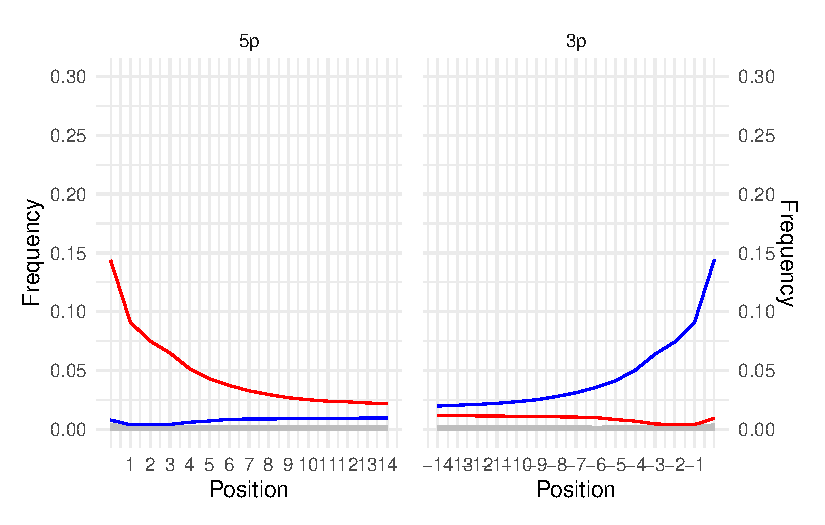
\includegraphics{double-stranded_files/figure-pdf/fig-double-stranded-smiley-1.pdf}

}

\caption{\label{fig-double-stranded-smiley}Example of a smiley plot of a
double stranded DNA library. Data taken from (Star et al. 2017). Damage
data generated using \href{/intro.qmd}{DamageProfiler} and plotted using
R and tidyverse packages (Wickham et al. 2019).}

\end{figure}

}

\end{minipage}%
%
\begin{minipage}[t]{0.50\linewidth}

{\centering 

\raisebox{-\height}{

\includegraphics{index_files/mediabag/512px-Salvador_dali_.jpg}

}

\caption{\label{fig-double-stranded-caricature}!!EXAMPLE NOT FINAL!!
snah Kritzler, CC0, via Wikimedia Commons}

}

\end{minipage}%

\end{figure}

This is the `classical' ancient DNA plot that you will see most often.
You expect to see a smooth curve from the beginning of the read
(position 1) to a flat line in the middle (e.g.~positions 10-25 in
mapDamage plots).

If you get such a plot in ancient DNA double-stranded libraries, this is
a good indication you have authentic ancient DNA!

\hypertarget{smiley-plot-of-single-stranded-dna-libraries}{%
\chapter{Smiley Plot of Single Stranded DNA
Libraries}\label{smiley-plot-of-single-stranded-dna-libraries}}

\hypertarget{smiley-plot-of-partial-udg-treatment-llibraries}{%
\chapter{Smiley plot of partial UDG treatment
lLibraries}\label{smiley-plot-of-partial-udg-treatment-llibraries}}

\part{Problematic Smiley Plots}

\hypertarget{smiley-plot-of-insufficient-reads}{%
\chapter{Smiley Plot of Insufficient
Reads}\label{smiley-plot-of-insufficient-reads}}

\bookmarksetup{startatroot}

\hypertarget{references}{%
\chapter*{References}\label{references}}
\addcontentsline{toc}{chapter}{References}

\markboth{References}{References}

\hypertarget{refs}{}
\begin{CSLReferences}{1}{0}
\leavevmode\vadjust pre{\hypertarget{ref-Briggs2007-ao}{}}%
Briggs, Adrian W, Udo Stenzel, Philip L F Johnson, Richard E Green,
Janet Kelso, Kay Prüfer, Matthias Meyer, et al. 2007. {``Patterns of
Damage in Genomic {DNA} Sequences from a Neandertal.''}
\emph{Proceedings of the National Academy of Sciences of the United
States of America} 104 (37): 14616--21.
\url{https://doi.org/10.1073/pnas.0704665104}.

\leavevmode\vadjust pre{\hypertarget{ref-Hubler2019-qw}{}}%
Hübler, Ron, Felix M Key, Christina Warinner, Kirsten I Bos, Johannes
Krause, and Alexander Herbig. 2019. {``{HOPS}: Automated Detection and
Authentication of Pathogen {DNA} in Archaeological Remains.''}
\emph{Genome Biology} 20 (1): 280.
\url{https://doi.org/10.1186/s13059-019-1903-0}.

\leavevmode\vadjust pre{\hypertarget{ref-Jonsson2013-zb}{}}%
Jónsson, Hákon, Aurélien Ginolhac, Mikkel Schubert, Philip L F Johnson,
and Ludovic Orlando. 2013. {``{mapDamage2}.0: Fast Approximate Bayesian
Estimates of Ancient {DNA} Damage Parameters.''} \emph{Bioinformatics}
29 (13): 1682--84. \url{https://doi.org/10.1093/bioinformatics/btt193}.

\leavevmode\vadjust pre{\hypertarget{ref-Neukamm2021-ul}{}}%
Neukamm, Judith, Alexander Peltzer, and Kay Nieselt. 2021.
{``{DamageProfiler}: Fast Damage Pattern Calculation for Ancient
{DNA}.''} \emph{Bioinformatics} 37 (20): 3652--53.
\url{https://doi.org/10.1093/bioinformatics/btab190}.

\leavevmode\vadjust pre{\hypertarget{ref-Star2017-cj}{}}%
Star, Bastiaan, Sanne Boessenkool, Agata T Gondek, Elena A Nikulina,
Anne Karin Hufthammer, Christophe Pampoulie, Halvor Knutsen, et al.
2017. {``Ancient {DNA} Reveals the Arctic Origin of Viking Age Cod from
Haithabu, Germany.''} \emph{Proceedings of the National Academy of
Sciences of the United States of America} 114 (34): 9152--57.
\url{https://doi.org/10.1073/pnas.1710186114}.

\leavevmode\vadjust pre{\hypertarget{ref-Wickham2019-ot}{}}%
Wickham, Hadley, Mara Averick, Jennifer Bryan, Winston Chang, Lucy
McGowan, Romain François, Garrett Grolemund, et al. 2019. {``Welcome to
the Tidyverse.''} \emph{Journal of Open Source Software} 4 (43): 1686.
\url{https://doi.org/10.21105/joss.01686}.

\end{CSLReferences}



\end{document}
